\documentclass[twocolumn]{article}
\usepackage[spanish]{babel}
\usepackage[utf8]{inputenc}
\usepackage{amssymb}
\usepackage{graphicx}
\usepackage{verbatim}
\usepackage{algorithmic}
\usepackage{enumitem}
\setlist{nolistsep}
\usepackage{fancyvrb}



\author{
Nombre:....................................... \\
    Departamento de Informática y Sistemas \\
    Universidad EAFIT \\
}
\title{
    Estructuras de Datos 2 - ST0247 \\
    Examen Parcial 1 
}
\date{
    Septiembre 14 de 2017
}

\begin{document}
\vspace{-5cm}
\maketitle


\section*{Criterios de calificación}

\begin{itemize}
\item Selección múltiple con única respuesta
\begin{itemize}
\item Respuesta correcta: 100\%
\item Respuesta incorrecta: 0\%
\end{itemize}

\item Completar código
\begin{itemize}
\item Respuesta correcta 100\%
\item Respuesta incorrecta o vacía 0\%
\end{itemize}
\end{itemize}

\vspace{1cm}

\textbf{NOTAS IMPORTANTES:}
\begin{itemize}
	\item Responda en la hoja de PREGUNTAS
	\item Marque la hoja de PREGUNTAS
\end{itemize}
\section{Fuerza bruta 30\%}
Un problema frecuente es buscar si una una cadena llamada \textbf{patrón} (\texttt{pat})
se encuentra dentro de otra cadena llamado \textbf{texto} (\texttt{txt}). Esto es lo que sucede 
en muchos programas cuando le damos \emph{Edición, Buscar}. El objetivo es
encontrar la posición en la que aparece por primera vez \texttt{pat} en \texttt{txt}.

Como un ejemplo, el patrón ``atr'' aparece dentro del texto ``patrón'' en la posición
$1$. Como otro ejemplo, el patrón ``mat'' no aparece en el texto ``patrón''. Cuando
no aparece, el algoritmo retorna la longitud del texto, es decir, en este caso, $5$.

Una forma de resolverlo es por fuerza bruta, probando todas las posibles posiciones
en las que \texttt{pat} puede aparecer dentro de \texttt{txt} como se muestra a continuación:

{\small
\begin{verbatim}
01 int indexOf(String pat, String txt) {
02  int m = pat.length();
03  int n = txt.length();
04  int i, j;
05  for (i = 0, j = 0; i < n && j < m; i++) {
06   if (txt.charAt(i) == pat.charAt(j)) j++;
07   else {
08     i = i - j;
09     j = 0;
10   }
11  }
12  if (j == m) return ______  // encontrado
13  else        return ______; // no encontrado
14 }
\end{verbatim}
}





     (10\%) Complete la línea 12\\


  \_\_\_\_\_\_\_\_\_\_\_\_ \\

       (10\%) Complete la línea 13\\


  \_\_\_\_\_\_\_\_\_\_\_\_ \\

     (10\%) ¿Cuál es la complejidad asintótica, para el peor de los casos, del algoritmo? (En términos de $n$ y $m$)\\


  O(\_\_\_\_)

    % public static int search2(String pat, String txt) {
    %     int m = pat.length();
    %     int n = txt.length();
    %     int i, j;
    %     for (i = 0, j = 0; i < n && j < m; i++) {
    %         if (txt.charAt(i) == pat.charAt(j)) j++;
    %         else {
    %             i -= j;
    %             j = 0;
    %         }
    %     }
    %     if (j == m) return i - m;    // found
    %     else        return n;        // not found
    % }

\textbf{Pista:} NO es $O(n!)$.

\section{Implementación grafos 20\%}
Considere el siguiente grafo:

\begin{center}
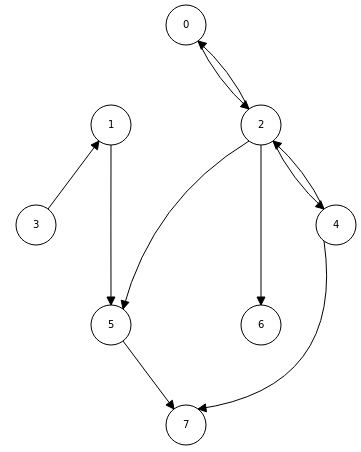
\includegraphics[scale=0.5]{grafin.png}
\end{center}

\begin{enumerate}[label=\Alph*]
\item (10\%) Complete la representación de \textbf{matrices de adyacencia}. Si no hay arco,
  deje el espacio en blanco. NO coloque ceros.

\begin{center}
\begin{tabular}{| c | c | c | c | c | c | c | c | c |}
\hline
  & 0 & 1 & 2 & 3 & 4 & 5 & 6 & 7 \\
\hline
0 &   &   & 1  &  &   &   &   &   \\
\hline
1 &   &   &   &   &   & 1  &   &   \\
\hline
2 &   &   &   &   &   &   &   &   \\
\hline
3 &   &   &   &   &   &   &   &   \\
\hline
4 &   &   &   &   &   &   &   &   \\
\hline
5 &   &   &   &   &   &   &   &   \\
\hline
6 &   &   &   &   &   &   &   &   \\
\hline
7 &   &   &   &   &   &   &   &   \\ 
\hline
\end{tabular}
\end{center}

\textbf{Pista:} NO coloque ceros.

	\item (10\%) Complete la representación de \textbf{listas de adyacencia}. Como
  el grafo no tiene pesos, sólo se colocan los sucesores en la lista de adyacencia.
  Los sucesores o vecinos son los vértices a los que se puede llegar a partir de
  un arco directamente, NO transitivamente. \\


$0 \rightarrow [2]$\\
$1 \rightarrow [5]$ \\
$2 \rightarrow$\\
$3 \rightarrow$\\
$4 \rightarrow$\\
$5 \rightarrow$\\
$6 \rightarrow$\\
$7 \rightarrow$\\


\end{enumerate}



\section{Recorridos de grafos 20\%}

Para el grafo anterior, complete la salida
que darían los siguientes algoritmos:


\begin{enumerate}[label=\Alph*]
	\item (10\%) Complete el orden en que se recorren los nodos usando \textbf{búsqueda en profundidad} (en Inglés DFS) a partir de cada nodo. Si hay varias opciones de recorrer el grafo con DFS, elija siempre el vértice más pequeño.\\


$0 \rightarrow$\\
$1 \rightarrow 5 \rightarrow  7$\\
$2 \rightarrow$\\
$3 \rightarrow$\\
$4 \rightarrow$\\
$5 \rightarrow$\\
$6 \rightarrow$\\
$7 \rightarrow$\\


\item (10\%) Complete el orden en que se recorren los nodos usando \textbf{búsqueda en amplitud} (en Inglés BFS) a partir de cada nodo. Si hay varias opciones de recorrer el grafo con BFS, elija siempre el vértice más pequeño.\\


$0 \rightarrow$\\
$1 \rightarrow 5 \rightarrow  7$\\
$2 \rightarrow$\\
$3 \rightarrow$\\
$4 \rightarrow$\\
$5 \rightarrow$\\
$6 \rightarrow$\\
$7 \rightarrow$\\


\end{enumerate}


\section{Backtracking 30\%}
% Considere el siguiente problema. Queremos determinar la \textbf{subsequencia común mas larga} (en inglés \textbf{LCS}) de dos cadenas $S_1$ y $S_2$. La \textbf{subsequencia común mas larga} de dos cadenas es la máxima cantidad de caracteres, no necesariamente contiguos, tales que $S_i = S_j$, $0 \leq i < |S_1|$ y $0 \leq j < |S_2|$. Por ejemplo la \textbf{subsequencia común mas larga} de $abcbcaaacb$ y $cabbcbac$ es $6$, $abbcac$. Otro ejemplo, la \textbf{subsequencia común mas larga} de $abcdef$ y $aghijk$ es $1$, $a$.
% \\

El problema de la \textbf{subsecuencia común más larga} es el siguiente. Dadas dos secuencias, encontrar la longitud de la secuencia más larga presente en ambas.
Una subsecuencia es una secuencia que aparece en el mismo orden relativo, pero no necesariamente de forma contigua. Como un ejemplo, ``abc'', ``abg'', ``bdf'',
``aeg'' y ``acefg'' son subsecuencias de ``abcdefg''. Entonces, para una cadena de longitud $n$ existen $2^n$ posibles subsecuencias. Este problema es utilizado
en la implementación del comando \texttt{diff}, para comparación de archivos, disponible en sistemas Unix.  También tiene muchas aplicaciones en bioinformática. \\

\noindent
Considere los siguientes ejemplos para el problema:
\begin{itemize}
\item Para ``ABCDGH'' y ``AEDFHR'' es ``ADH'' y su longitud es 3.
\item Para ``AGGTAB'' y ``GXTXAYB'' es ``GTAB'' y su longitud es 4.\\
\end{itemize}

Una forma de resolver este problema es usando \emph{backtracking}, como un ejemplo, para las cadenas  ``AXYT'' y  ``AYZX'', dada una función recursiva \texttt{lcs} 
que resuelve el problema, se obtendría el siguiente árbol (parcial) de recursión:

{\scriptsize
\begin{Verbatim}[commandchars=\\\{\},codes={\catcode`$=3\catcode`_=8}]
                 lcs("AXYT", "AYZX")
                 /                 \textbackslash
    lcs("AXY", "AYZX")            lcs("AXYT", "AYZ")
\_\_\_\_\_\_\_\_\_\_\_\_\_\_\_\_\_\_\_\_\_\_\_\_\_\_\_\_\_\_\_\_\_\_\_\_\_\_\_\_\_\_\_\_\_\_\_\_\_\_\_\_\_\_\_\_\_\_\_\_\_\_\_\_\_\_\_\_\_\_\_\_
    lcs("AXY", "AYZX")          
      /            \textbackslash               
lcs("AX", "AYZX") \textbf{lcs("AXY", "AYZ")}
\_\_\_\_\_\_\_\_\_\_\_\_\_\_\_\_\_\_\_\_\_\_\_\_\_\_\_\_\_\_\_\_\_\_\_\_\_\_\_\_\_\_\_\_\_\_\_\_\_\_\_\_\_\_\_\_\_\_\_\_\_\_\_\_\_\_\_\_\_\_\_\_\_
    lcs("AXYT", "AYZ")
     /             \textbackslash
\textbf{lcs("AXY", "AYZ")} lcs("AXYT", "AY")
\end{Verbatim}
}



Al siguiente código le faltan algunas lineas, complétalas por favor.

{\footnotesize
\begin{verbatim}











01 private int lcs(int i, int j, String s1, String s2){
02     if(i == 0 || j == 0){
03         return 0;   
04     }
05     boolean prev = i < s1.length() && j < s2.length();
06     if(prev && s1.charAt(i) == s2.charAt(j)){
07         return ______+ lcs(i - 1, j - 1, s1, s2);
08     }
09     int ni = lcs(i - 1, j, s1, s2);
10     int nj = lcs(i, j - 1, s1, s2);
11     return Math.max(_____, _____);
12 }
13 public int lcs(String s1, String s2){
14     return lcs(s1.length(), s2.length(), s1, s2);
15 }
\end{verbatim}
}

 (10\%) Linea 7  \_\_\_\_\_\_\_\_\_\_\_\_ \\

 (10\%) Linea 11 \_\_\_\_\_\_\_\_\_\_\_\_, \_\_\_\_\_\_\_\_\_\_\_\_ \\

Y complete la complejidad por favor \\
 
 (10\%) Suponga que $n$ es la suma de la longitud de las dos cadenas. El algoritmo \texttt{lcs} ejecuta, en el
 peor de los casos, $T(n)$ = \_\_\_\_\_\_\_\_\_\_\_\_\_\_ instrucciones. \\

\end{document}
